\documentclass{standalone}
\usepackage{tikz}
\usetikzlibrary{patterns, positioning}
\usepackage[sfdefault]{ClearSans} %% option 'sfdefault' activates Clear Sans as the default text font
\usepackage[T1]{fontenc}

\begin{document}
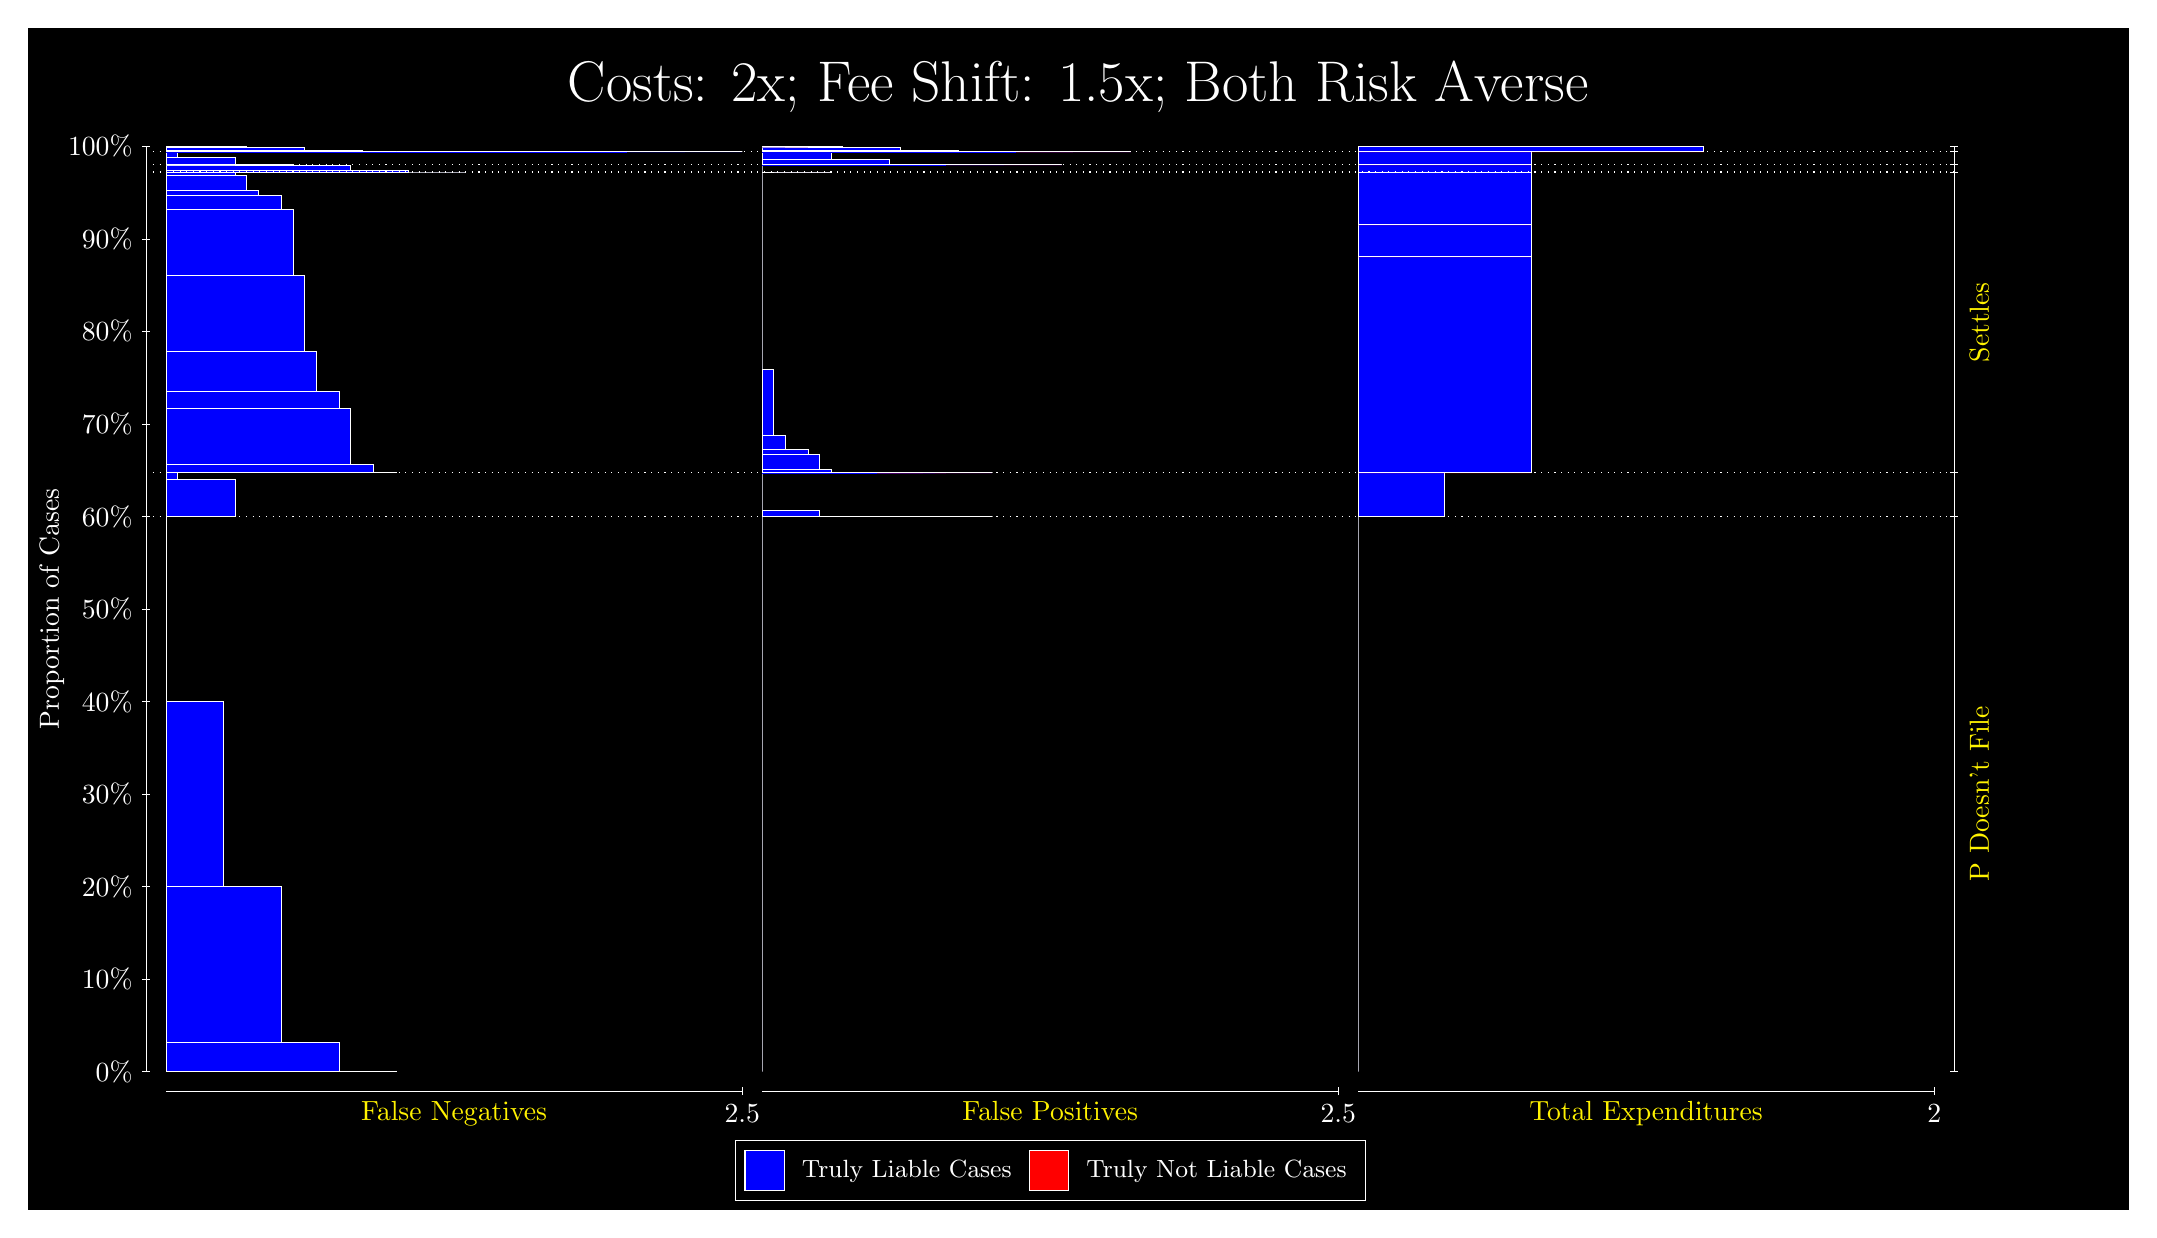
\begin{tikzpicture}
\draw[fill=black] (0,0) rectangle (26.667,15);
\draw[text=white] (0,13.5) rectangle (26.667,15) node[midway] {\huge Costs: 2x; Fee Shift: 1.5x; Both Risk Averse};
\draw[white, very thin] (1.5,1.75) -- (1.5,13.5);
\node[rotate=90, text=white, anchor=center] at (0.3, 7.625) {Proportion of Cases};
\draw[white, very thin] (1.45,1.75) -- (1.55,1.75);
\node[text=white, anchor=east] at (1.45, 1.75) {0\%};
\draw[white, very thin] (1.45,2.925) -- (1.55,2.925);
\node[text=white, anchor=east] at (1.45, 2.925) {10\%};
\draw[white, very thin] (1.45,4.1) -- (1.55,4.1);
\node[text=white, anchor=east] at (1.45, 4.1) {20\%};
\draw[white, very thin] (1.45,5.275) -- (1.55,5.275);
\node[text=white, anchor=east] at (1.45, 5.275) {30\%};
\draw[white, very thin] (1.45,6.45) -- (1.55,6.45);
\node[text=white, anchor=east] at (1.45, 6.45) {40\%};
\draw[white, very thin] (1.45,7.625) -- (1.55,7.625);
\node[text=white, anchor=east] at (1.45, 7.625) {50\%};
\draw[white, very thin] (1.45,8.8) -- (1.55,8.8);
\node[text=white, anchor=east] at (1.45, 8.8) {60\%};
\draw[white, very thin] (1.45,9.975) -- (1.55,9.975);
\node[text=white, anchor=east] at (1.45, 9.975) {70\%};
\draw[white, very thin] (1.45,11.15) -- (1.55,11.15);
\node[text=white, anchor=east] at (1.45, 11.15) {80\%};
\draw[white, very thin] (1.45,12.325) -- (1.55,12.325);
\node[text=white, anchor=east] at (1.45, 12.325) {90\%};
\draw[white, very thin] (1.45,13.5) -- (1.55,13.5);
\node[text=white, anchor=east] at (1.45, 13.5) {100\%};

\draw[white, very thin] (24.457,1.75) -- (24.457,13.5);
\draw[white, very thin] (24.407,1.75) -- (24.507,1.75);
\node[anchor=west] at (24.407, 1.75) {};
\draw[white, very thin] (24.407,8.8012) -- (24.507,8.8012);
\node[anchor=west] at (24.407, 8.8012) {};
\draw[white, very thin] (24.407,9.3551) -- (24.507,9.3551);
\node[anchor=west] at (24.407, 9.3551) {};
\draw[white, very thin] (24.407,13.174) -- (24.507,13.174);
\node[anchor=west] at (24.407, 13.174) {};
\draw[white, very thin] (24.407,13.266) -- (24.507,13.266);
\node[anchor=west] at (24.407, 13.266) {};
\draw[white, very thin] (24.407,13.431) -- (24.507,13.431);
\node[anchor=west] at (24.407, 13.431) {};
\draw[white, very thin] (24.407,13.5) -- (24.507,13.5);
\node[anchor=west] at (24.407, 13.5) {};

\draw[white, very thin, fill=blue] (1.75,1.75) rectangle (4.6775,1.7538);
\draw[white, very thin, fill=blue] (1.75,1.7538) rectangle (3.9457,2.1271);
\draw[white, very thin, fill=blue] (1.75,2.1271) rectangle (3.2138,4.1043);
\draw[white, very thin, fill=blue] (1.75,4.1043) rectangle (2.4819,6.4512);
\draw[white, very thin, fill=red] (1.75,6.4512) rectangle (1.75,6.4512);
\draw[white, very thin, fill=blue] (1.75,6.4512) rectangle (1.75,8.8012);
\draw[white, very thin, fill=blue] (1.75,8.8012) rectangle (2.6283,9.2771);
\draw[white, very thin, fill=blue] (1.75,9.2771) rectangle (1.8964,9.3549);
\draw[white, very thin, fill=red] (1.75,9.3549) rectangle (1.75,9.3549);
\draw[white, very thin, fill=blue] (1.75,9.3549) rectangle (1.75,9.3551);
\draw[white, very thin, fill=blue] (1.75,9.3551) rectangle (4.6775,9.3587);
\draw[white, very thin, fill=blue] (1.75,9.3587) rectangle (4.3848,9.457);
\draw[white, very thin, fill=blue] (1.75,9.457) rectangle (4.092,10.171);
\draw[white, very thin, fill=blue] (1.75,10.171) rectangle (3.9457,10.393);
\draw[white, very thin, fill=blue] (1.75,10.393) rectangle (3.6529,10.897);
\draw[white, very thin, fill=blue] (1.75,10.897) rectangle (3.5065,11.859);
\draw[white, very thin, fill=blue] (1.75,11.859) rectangle (3.3602,12.699);
\draw[white, very thin, fill=blue] (1.75,12.699) rectangle (3.2138,12.88);
\draw[white, very thin, fill=blue] (1.75,12.88) rectangle (2.921,12.946);
\draw[white, very thin, fill=blue] (1.75,12.946) rectangle (2.7746,13.131);
\draw[white, very thin, fill=blue] (1.75,13.131) rectangle (2.6283,13.172);
\draw[white, very thin, fill=blue] (1.75,13.172) rectangle (2.4819,13.172);
\draw[white, very thin, fill=blue] (1.75,13.172) rectangle (2.1891,13.173);
\draw[white, very thin, fill=blue] (1.75,13.173) rectangle (2.0428,13.174);
\draw[white, very thin, fill=blue] (1.75,13.174) rectangle (1.8964,13.174);
\draw[white, very thin, fill=red] (1.75,13.174) rectangle (1.75,13.174);
\draw[white, very thin, fill=blue] (1.75,13.174) rectangle (1.75,13.174);
\draw[white, very thin, fill=blue] (1.75,13.174) rectangle (5.5558,13.174);
\draw[white, very thin, fill=blue] (1.75,13.174) rectangle (4.8239,13.195);
\draw[white, very thin, fill=blue] (1.75,13.195) rectangle (4.092,13.264);
\draw[white, very thin, fill=blue] (1.75,13.264) rectangle (3.3602,13.266);
\draw[white, very thin, fill=blue] (1.75,13.266) rectangle (2.6283,13.266);
\draw[white, very thin, fill=red] (1.75,13.266) rectangle (1.75,13.266);
\draw[white, very thin, fill=blue] (1.75,13.266) rectangle (2.6283,13.356);
\draw[white, very thin, fill=blue] (1.75,13.356) rectangle (1.8964,13.43);
\draw[white, very thin, fill=red] (1.75,13.43) rectangle (1.75,13.43);
\draw[white, very thin, fill=blue] (1.75,13.43) rectangle (1.75,13.431);
\draw[white, very thin, fill=blue] (1.75,13.431) rectangle (9.0689,13.431);
\draw[white, very thin, fill=blue] (1.75,13.431) rectangle (8.337,13.431);
\draw[white, very thin, fill=blue] (1.75,13.431) rectangle (7.6051,13.433);
\draw[white, very thin, fill=blue] (1.75,13.433) rectangle (6.8732,13.435);
\draw[white, very thin, fill=blue] (1.75,13.435) rectangle (6.1413,13.435);
\draw[white, very thin, fill=blue] (1.75,13.435) rectangle (5.7022,13.435);
\draw[white, very thin, fill=blue] (1.75,13.435) rectangle (5.4094,13.435);
\draw[white, very thin, fill=blue] (1.75,13.435) rectangle (4.9703,13.435);
\draw[white, very thin, fill=blue] (1.75,13.435) rectangle (4.6775,13.435);
\draw[white, very thin, fill=blue] (1.75,13.435) rectangle (4.2384,13.449);
\draw[white, very thin, fill=blue] (1.75,13.449) rectangle (3.5065,13.484);
\draw[white, very thin, fill=blue] (1.75,13.484) rectangle (2.7746,13.5);
\draw[white, very thin, fill=blue] (1.75,13.5) rectangle (2.0428,13.5);
\draw[white, very thin, fill=red] (1.75,13.5) rectangle (1.75,13.5);
\draw[white, very thin, fill=blue] (1.75,13.5) rectangle (1.75,13.5);
\draw[white, very thin, fill=red] (9.3189,1.75) rectangle (9.3189,1.75);
\draw[white, very thin, fill=blue] (9.3189,1.75) rectangle (9.3189,8.8012);
\draw[white, very thin, fill=red] (9.3189,8.8012) rectangle (12.246,8.8012);
\draw[white, very thin, fill=blue] (9.3189,8.8012) rectangle (12.246,8.8012);
\draw[white, very thin, fill=blue] (9.3189,8.8012) rectangle (11.515,8.8012);
\draw[white, very thin, fill=blue] (9.3189,8.8012) rectangle (10.783,8.8013);
\draw[white, very thin, fill=blue] (9.3189,8.8013) rectangle (10.051,8.8791);
\draw[white, very thin, fill=blue] (9.3189,8.8791) rectangle (9.3189,9.3551);
\draw[white, very thin, fill=red] (9.3189,9.3551) rectangle (12.246,9.3551);
\draw[white, very thin, fill=blue] (9.3189,9.3551) rectangle (12.246,9.3551);
\draw[white, very thin, fill=red] (9.3189,9.3551) rectangle (11.661,9.3551);
\draw[white, very thin, fill=blue] (9.3189,9.3551) rectangle (11.661,9.3551);
\draw[white, very thin, fill=blue] (9.3189,9.3551) rectangle (11.515,9.3551);
\draw[white, very thin, fill=red] (9.3189,9.3551) rectangle (11.368,9.3551);
\draw[white, very thin, fill=blue] (9.3189,9.3551) rectangle (11.368,9.3551);
\draw[white, very thin, fill=red] (9.3189,9.3551) rectangle (11.075,9.3551);
\draw[white, very thin, fill=blue] (9.3189,9.3551) rectangle (11.075,9.3551);
\draw[white, very thin, fill=blue] (9.3189,9.3551) rectangle (10.929,9.3551);
\draw[white, very thin, fill=blue] (9.3189,9.3551) rectangle (10.783,9.3566);
\draw[white, very thin, fill=blue] (9.3189,9.3566) rectangle (10.636,9.3567);
\draw[white, very thin, fill=blue] (9.3189,9.3567) rectangle (10.344,9.3571);
\draw[white, very thin, fill=blue] (9.3189,9.3571) rectangle (10.197,9.3977);
\draw[white, very thin, fill=blue] (9.3189,9.3977) rectangle (10.051,9.5829);
\draw[white, very thin, fill=blue] (9.3189,9.5829) rectangle (9.9044,9.6492);
\draw[white, very thin, fill=blue] (9.3189,9.6492) rectangle (9.6116,9.8306);
\draw[white, very thin, fill=blue] (9.3189,9.8306) rectangle (9.4652,10.671);
\draw[white, very thin, fill=blue] (9.3189,10.671) rectangle (9.3189,13.174);
\draw[white, very thin, fill=red] (9.3189,13.174) rectangle (10.197,13.174);
\draw[white, very thin, fill=blue] (9.3189,13.174) rectangle (10.197,13.174);
\draw[white, very thin, fill=blue] (9.3189,13.174) rectangle (9.4652,13.176);
\draw[white, very thin, fill=blue] (9.3189,13.176) rectangle (9.3189,13.266);
\draw[white, very thin, fill=red] (9.3189,13.266) rectangle (13.125,13.266);
\draw[white, very thin, fill=blue] (9.3189,13.266) rectangle (13.125,13.266);
\draw[white, very thin, fill=blue] (9.3189,13.266) rectangle (12.393,13.266);
\draw[white, very thin, fill=blue] (9.3189,13.266) rectangle (11.661,13.267);
\draw[white, very thin, fill=blue] (9.3189,13.267) rectangle (10.929,13.341);
\draw[white, very thin, fill=blue] (9.3189,13.341) rectangle (10.197,13.431);
\draw[white, very thin, fill=red] (9.3189,13.431) rectangle (14.003,13.431);
\draw[white, very thin, fill=blue] (9.3189,13.431) rectangle (14.003,13.431);
\draw[white, very thin, fill=red] (9.3189,13.431) rectangle (13.271,13.431);
\draw[white, very thin, fill=blue] (9.3189,13.431) rectangle (13.271,13.431);
\draw[white, very thin, fill=red] (9.3189,13.431) rectangle (12.539,13.431);
\draw[white, very thin, fill=blue] (9.3189,13.431) rectangle (12.539,13.432);
\draw[white, very thin, fill=blue] (9.3189,13.432) rectangle (11.807,13.447);
\draw[white, very thin, fill=red] (9.3189,13.447) rectangle (11.807,13.447);
\draw[white, very thin, fill=blue] (9.3189,13.447) rectangle (11.807,13.447);
\draw[white, very thin, fill=blue] (9.3189,13.447) rectangle (11.075,13.482);
\draw[white, very thin, fill=blue] (9.3189,13.482) rectangle (11.075,13.482);
\draw[white, very thin, fill=blue] (9.3189,13.482) rectangle (10.344,13.494);
\draw[white, very thin, fill=blue] (9.3189,13.494) rectangle (10.344,13.496);
\draw[white, very thin, fill=red] (9.3189,13.496) rectangle (9.9044,13.496);
\draw[white, very thin, fill=blue] (9.3189,13.496) rectangle (9.9044,13.496);
\draw[white, very thin, fill=blue] (9.3189,13.496) rectangle (9.6116,13.496);
\draw[white, very thin, fill=blue] (9.3189,13.496) rectangle (9.6116,13.496);
\draw[white, very thin, fill=red] (9.3189,13.496) rectangle (9.3189,13.496);
\draw[white, very thin, fill=blue] (9.3189,13.496) rectangle (9.3189,13.5);
\draw[white, very thin, fill=red] (16.888,1.75) rectangle (16.888,1.75);
\draw[white, very thin, fill=blue] (16.888,1.75) rectangle (16.888,8.8012);
\draw[white, very thin, fill=red] (16.888,8.8012) rectangle (17.986,8.8012);
\draw[white, very thin, fill=blue] (16.888,8.8012) rectangle (17.986,9.3551);
\draw[white, very thin, fill=red] (16.888,9.3551) rectangle (19.083,9.3551);
\draw[white, very thin, fill=blue] (16.888,9.3551) rectangle (19.083,12.098);
\draw[white, very thin, fill=red] (16.888,12.098) rectangle (19.083,12.098);
\draw[white, very thin, fill=blue] (16.888,12.098) rectangle (19.083,12.505);
\draw[white, very thin, fill=red] (16.888,12.505) rectangle (19.083,12.505);
\draw[white, very thin, fill=blue] (16.888,12.505) rectangle (19.083,13.174);
\draw[white, very thin, fill=red] (16.888,13.174) rectangle (19.083,13.174);
\draw[white, very thin, fill=blue] (16.888,13.174) rectangle (19.083,13.266);
\draw[white, very thin, fill=red] (16.888,13.266) rectangle (19.083,13.266);
\draw[white, very thin, fill=blue] (16.888,13.266) rectangle (19.083,13.431);
\draw[white, very thin, fill=red] (16.888,13.431) rectangle (21.279,13.431);
\draw[white, very thin, fill=blue] (16.888,13.431) rectangle (21.279,13.498);
\draw[white, very thin, fill=red] (16.888,13.498) rectangle (21.279,13.498);
\draw[white, very thin, fill=blue] (16.888,13.498) rectangle (21.279,13.5);
\draw[white, dotted] (1.5,8.8012) -- (24.457,8.8012);
\draw[white, dotted] (1.5,9.3551) -- (24.457,9.3551);
\draw[white, dotted] (1.5,13.174) -- (24.457,13.174);
\draw[white, dotted] (1.5,13.266) -- (24.457,13.266);
\draw[white, dotted] (1.5,13.431) -- (24.457,13.431);
\draw[white, very thin] (1.75,1.5) -- (9.0689,1.5);
\node[text=yellow, anchor=north] at (5.4094, 1.5) {False Negatives};
\draw[white, very thin] (9.0689,1.45) -- (9.0689,1.55);
\node[text=white, anchor=north] at (9.0689, 1.45) {2.5};

\draw[white, very thin] (9.3189,1.5) -- (16.638,1.5);
\node[text=yellow, anchor=north] at (12.978, 1.5) {False Positives};
\draw[white, very thin] (16.638,1.45) -- (16.638,1.55);
\node[text=white, anchor=north] at (16.638, 1.45) {2.5};

\draw[white, very thin] (16.888,1.5) -- (24.207,1.5);
\node[text=yellow, anchor=north] at (20.547, 1.5) {Total Expenditures};
\draw[white, very thin] (24.207,1.45) -- (24.207,1.55);
\node[text=white, anchor=north] at (24.207, 1.45) {2};

\node[text=yellow, centered, rotate=90] at (24.777, 5.2756) {P Doesn't File};

\node[text=yellow, centered, rotate=90] at (24.777, 11.265) {Settles};




\draw (12.978300999999998,1.5) node[draw=none] (baseCoordinate) {};
\begin{scope}[align=center]
        \matrix[scale=0.5, draw=white, below=0.5cm of baseCoordinate, nodes={draw}, column sep=0.1cm]{
            \node[rectangle, draw, minimum width=0.5cm, minimum height=0.5cm, fill=blue] {}; &
            \node[draw=none, font=\small, text=white] (B) {Truly Liable Cases}; &
            \node[rectangle, draw, minimum width=0.5cm, minimum height=0.5cm, fill=red] {}; &
            \node[draw=none, font=\small, text=white] (B) {Truly Not Liable Cases}; \\
            };
\end{scope}

\end{tikzpicture}
\end{document}